\begin{figure}[t!]
	% \vspace{-12pt}
	 \renewcommand{\arraystretch}{0.4}
	\centering
	\resizebox{1\columnwidth}{!}{%
	\begin{tabular}{@{}c@{\hskip .1cm}c@{\hskip .1cm}c@{\hskip .1cm}c@{\hskip .1cm}c@{\hskip .1cm}c@{}}
	    \multicolumn{2}{c}{\large (i) Input Frame} & \multicolumn{2}{c}{\large (ii) INR 3D Generation} & \multicolumn{2}{c}{\large (iii) INR BEV Layout} \\
    	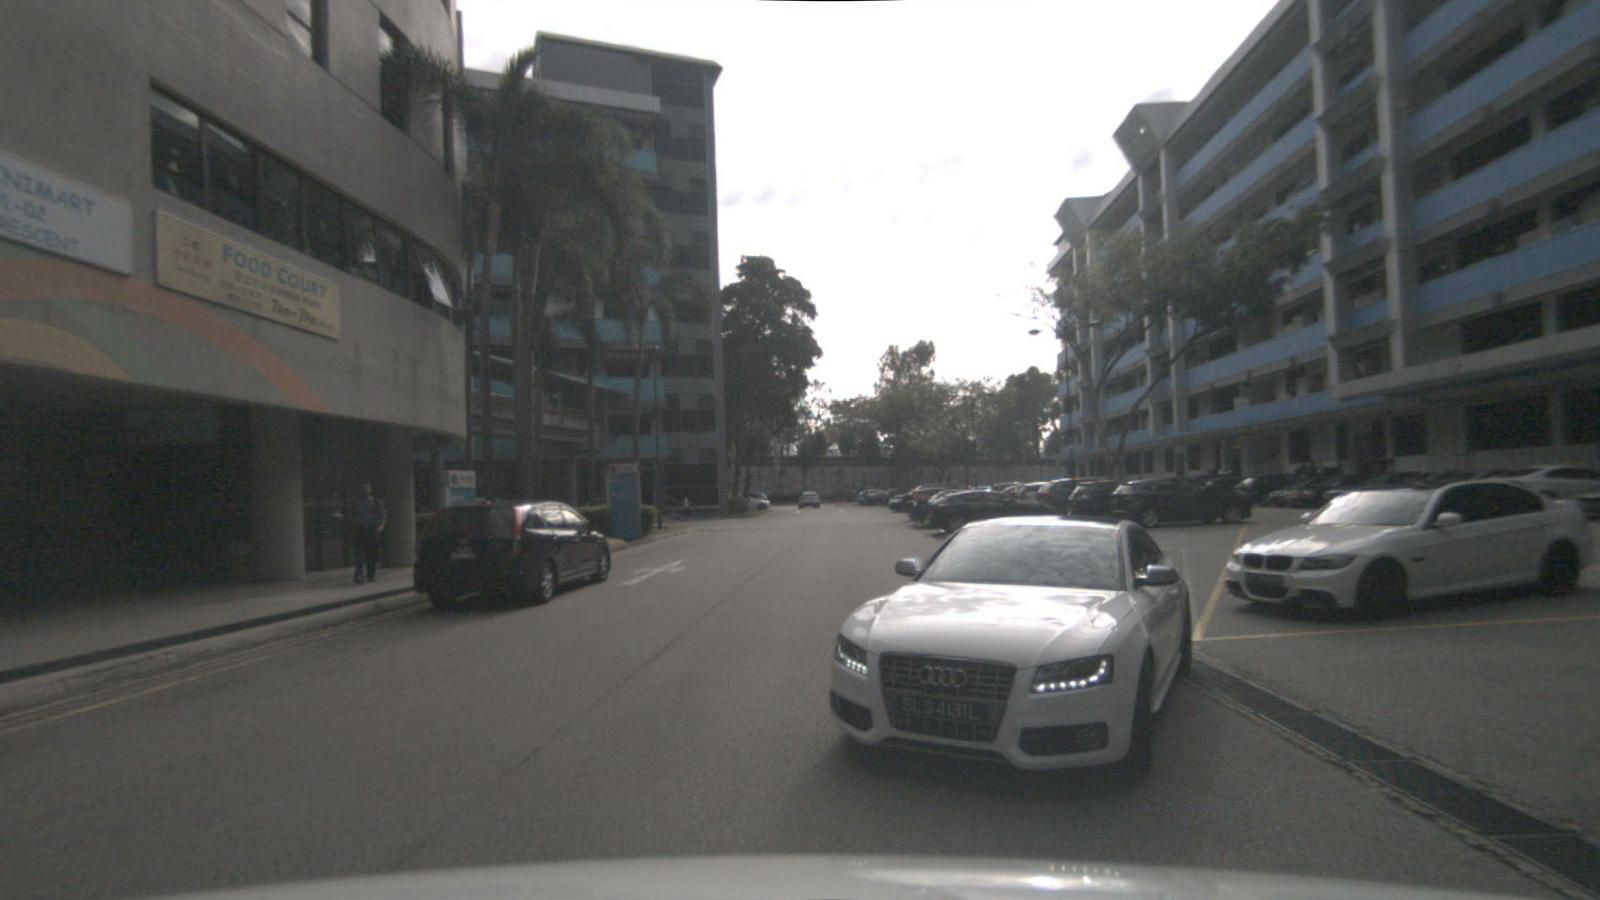
\includegraphics[width=.31\columnwidth, trim={0cm 0cm 0cm 0cm},clip]{fig/BEV_and_3D/scene1/nusc_sc_3_cam_5_f9_gt.png}&
         	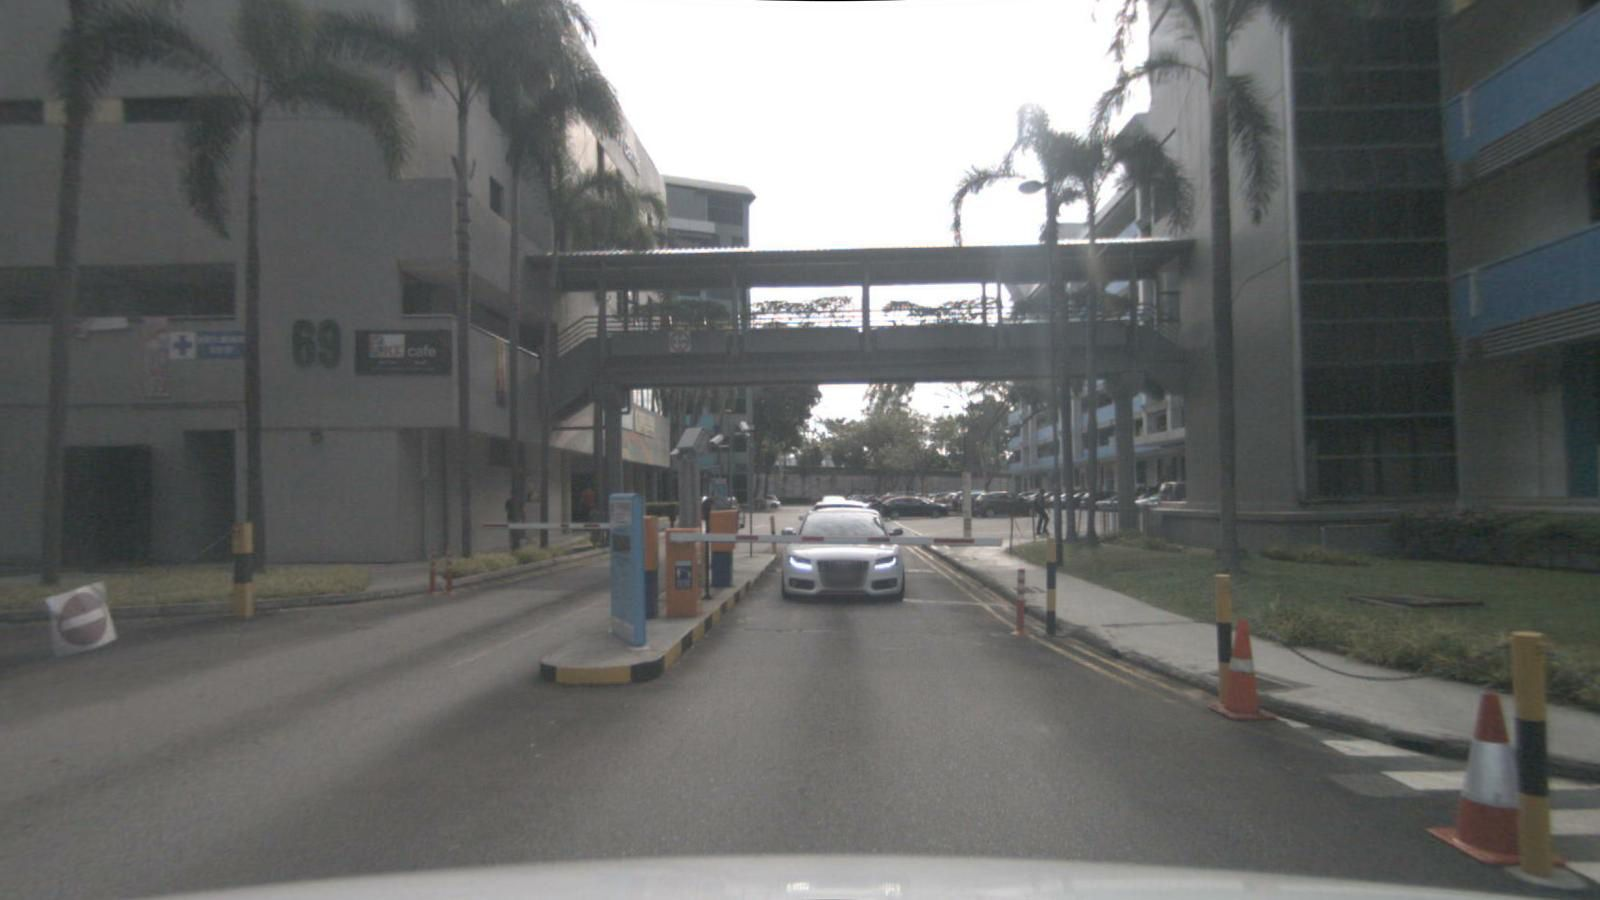
\includegraphics[width=.31\columnwidth, trim={26cm 6.7cm 12.5cm 15cm},clip]{fig/BEV_and_3D/scene2/gt_img.png}&
    	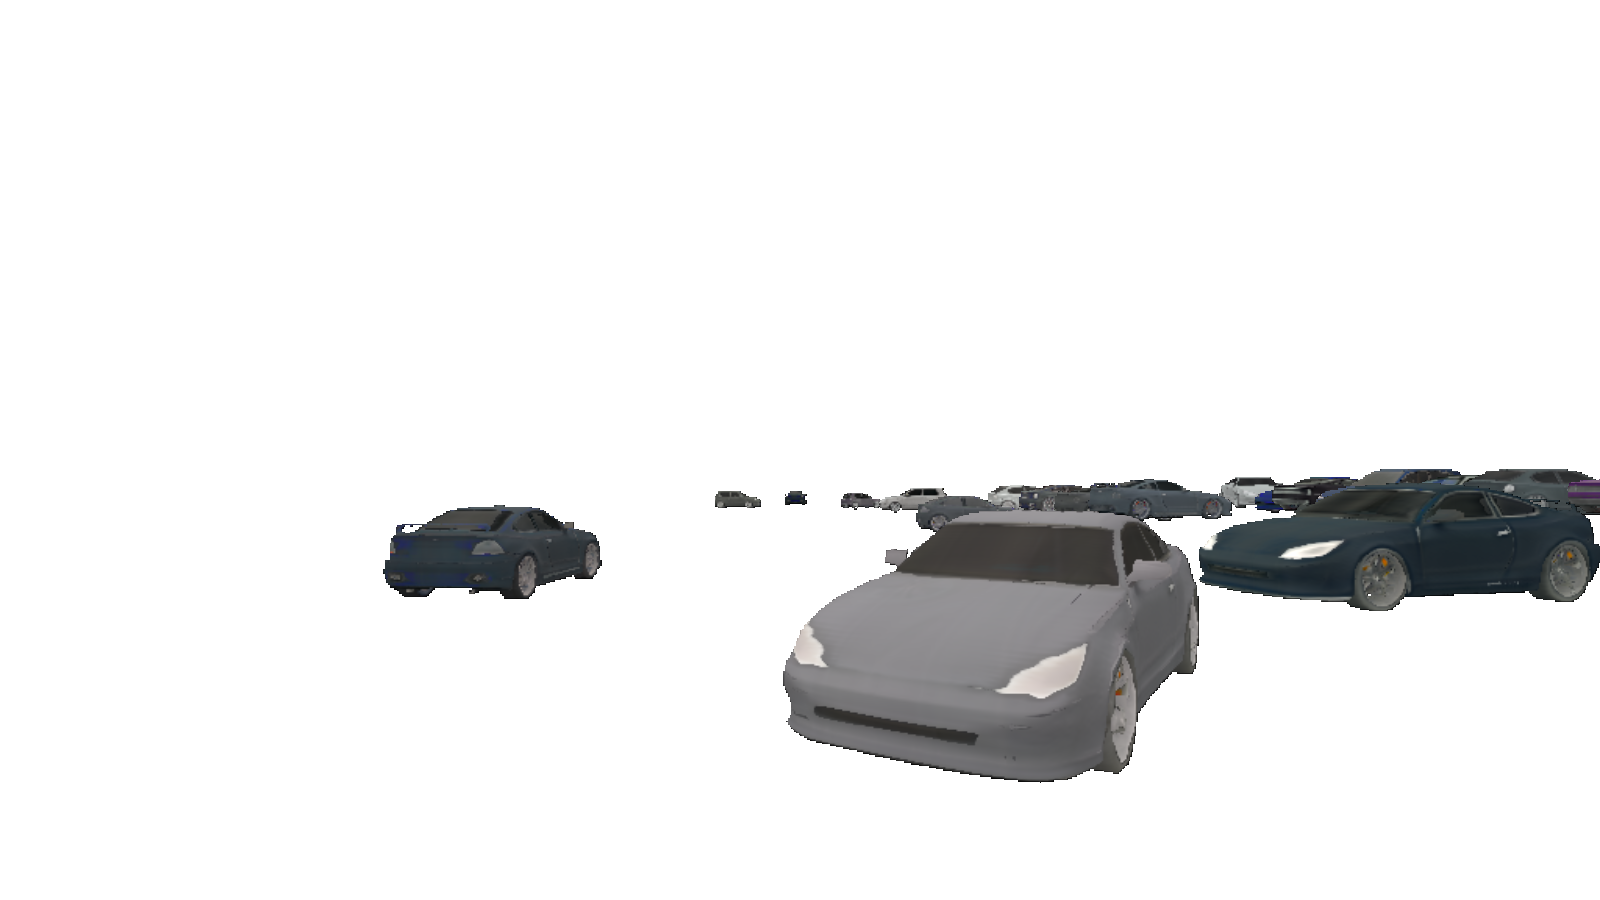
\includegraphics[width=.31\columnwidth, trim={0cm 0cm 0cm 0cm},clip]{fig/BEV_and_3D/scene1/sc_3_cam5_f9_rgb_out.png}&
         	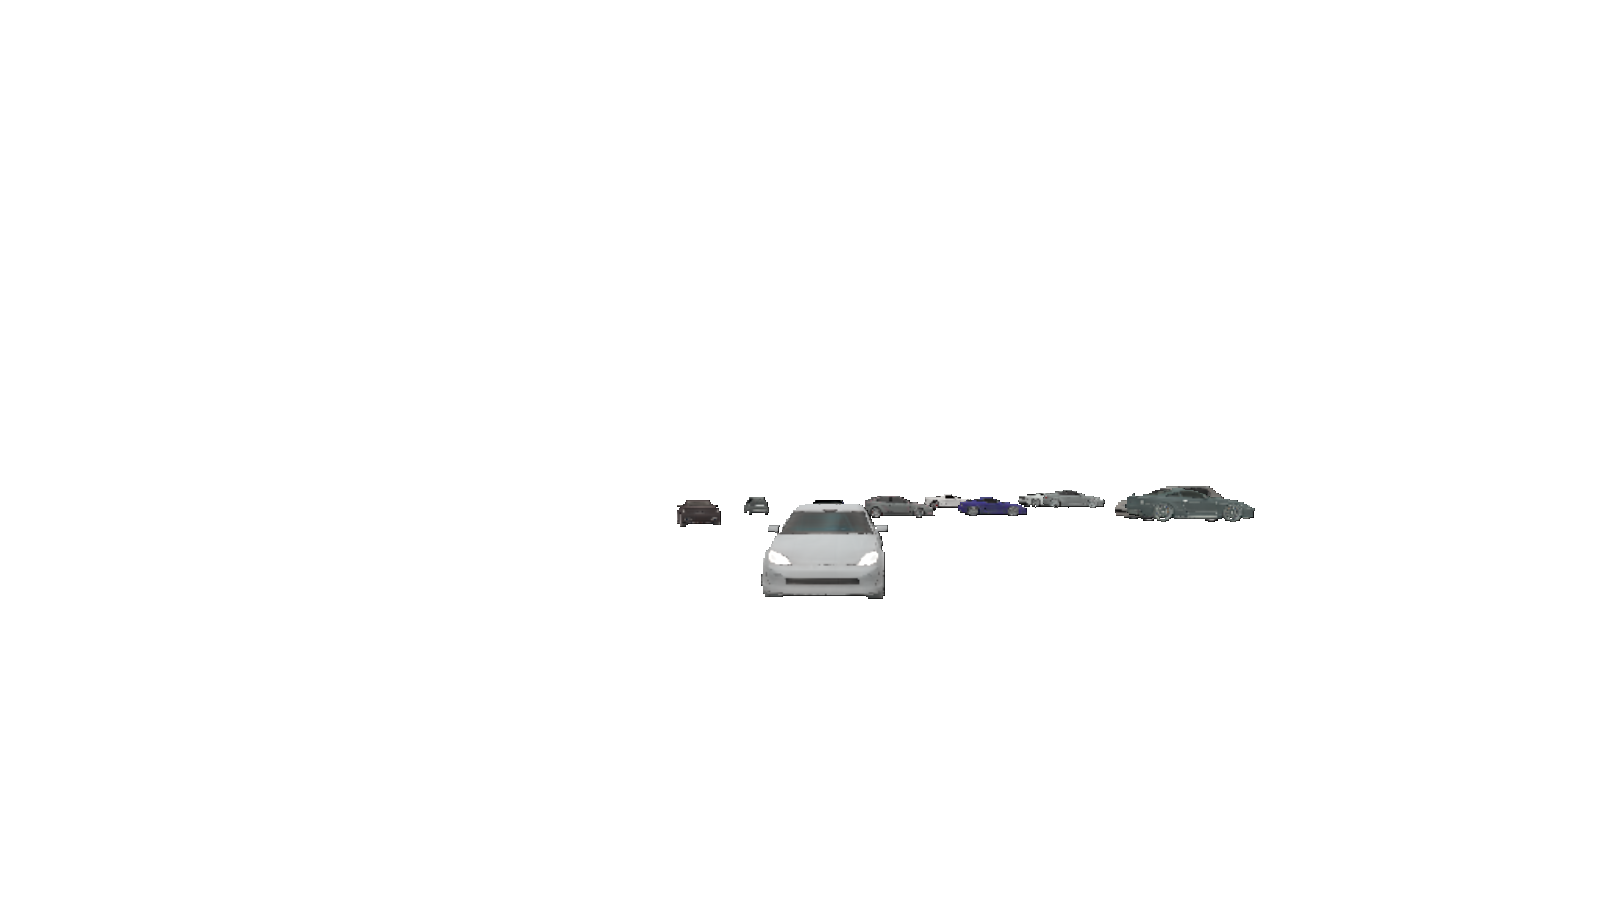
\includegraphics[width=.31\columnwidth, trim={26cm 6.7cm 12.5cm 15cm},clip]{fig/BEV_and_3D/scene2/rgb_out.png}&
    	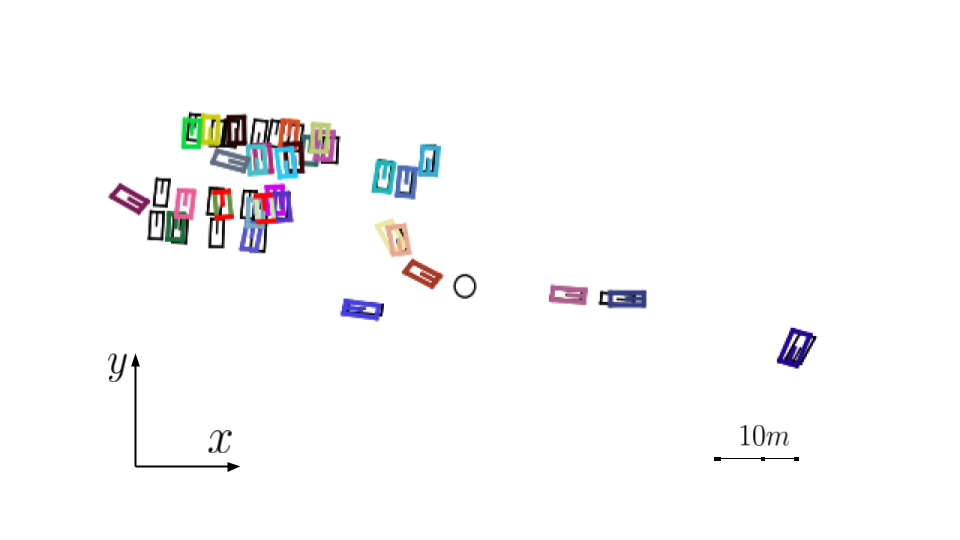
\includegraphics[width=.31\columnwidth, trim={2.1cm 2cm 1.9cm 2cm},clip]{fig/BEV_and_3D/BEV_axis_1.png}&
     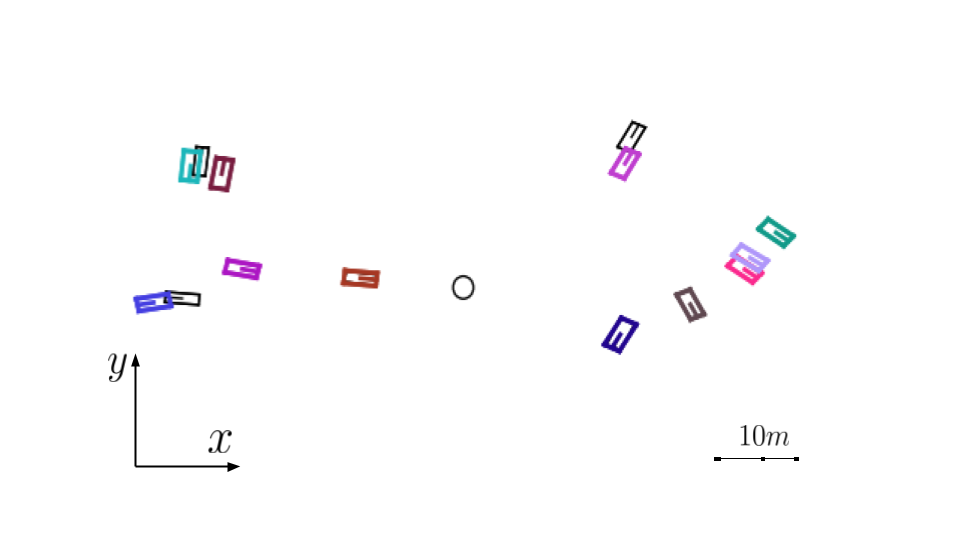
\includegraphics[width=.31\columnwidth, trim={2.1cm 2cm 1.9cm 2cm},clip]{fig/BEV_and_3D/BEV_axis_2.png}\\
     \textbf{\large (a)} & \textbf{\large (b)} & \textbf{\large (a)} & \textbf{\large (b)} & \textbf{\large (a)} & \textbf{\large (b)} \\
    \end{tabular}}
    \vspace*{-6pt}
\caption{\textbf{Layout Generation Through Inverse Rendering.} From left to right, we show (i) observed image from a single camera for two scenes (a, b), (ii) test-time optimized inverse rendered (IR) objects of class ``car'', and (iii) Bird's Eye View (BEV) layout of the scene. In the BEV layout, black boxes represent ground truth, and the colored boxes represent our predicted BEV boxes. The bottom shows a zoomed-in region at a 60 m distance (see BEV layout). Even in this setting, our method accurately recovers the 3D location, orientation, size, coarse appearance, and shape of the objects.} 
\label{fig:BEV3D_fig}
\vspace*{-16pt}
\end{figure}

